\section{Advanced architecture development}
<<<<<<< HEAD
=======
In this section is analyzed the design of the same IIR filter seen previously but with an advanced architecture, developed with the J-look-ahead technique. The basic equation of the filter is the following:
$$ y[n] = b_0x[n] + b_1x[n-1] + a_1y[n-1]$$

The J-look-ahead technique involves rewriting the equation by replacing the term $y[n-1]$ by evaluating it as a function of $y[n-2]$.
$$ y[n-1] = b_0x[n-1] + b_1x[n-2] + a_1y[n-2]$$

Then it is possible to replace the result obtained in the starting equation:
$$ y[n] = b_0x[n] + b_1x[n-1] + a_1(b_0x[n-1] + b_1x[n-2] + a_1y[n-2])$$
$$ y[n] = b_0x[n] + (b_1 + a_1)x[n-1] + a_1b_1x[n-2] + {a_1}^{2}y[n-2]$$

While keeping the classical architecture of the IIR direct form II filter, the resulting equation can be implemented through the scheme of a second-order filter.

\begin{figure}[h]
	\center
	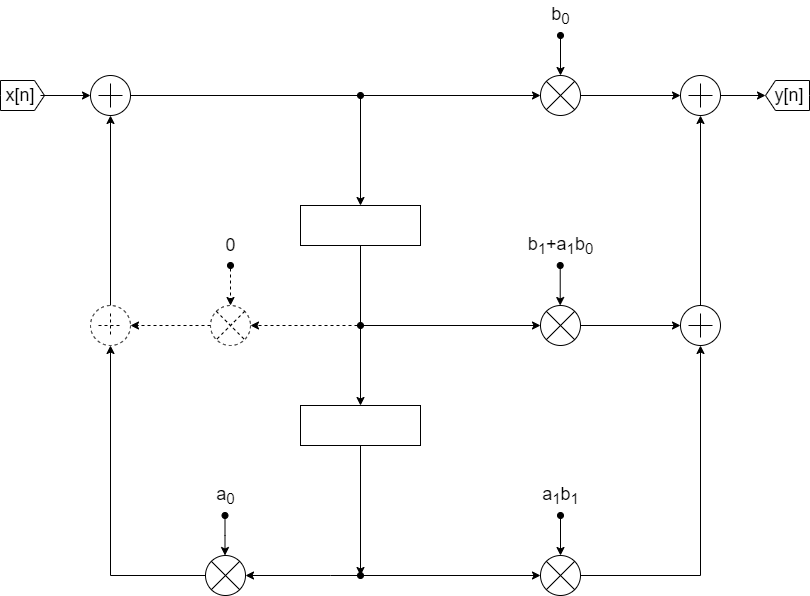
\includegraphics[width=0.65\textwidth]{IIR_2.png}
	\caption{IIR filter with J-look-ahead technique}
	\label{fig:IIR_advanced}
\end{figure}

This structure can be, as opposed to the previous version, improved in terms of performance. The critical path of this scheme consists of 4 combinatorial blocks, two multipliers and two adders, though by means of the appropriate transformations it is possible to reduce the longest combinatorial path.  In \autoref{fig:IIR_advanced_2} it has been identified the first cut-set that allows to move the register by changing the length of the critical path from 4 to 3.

\begin{figure}[htb]
	\center
	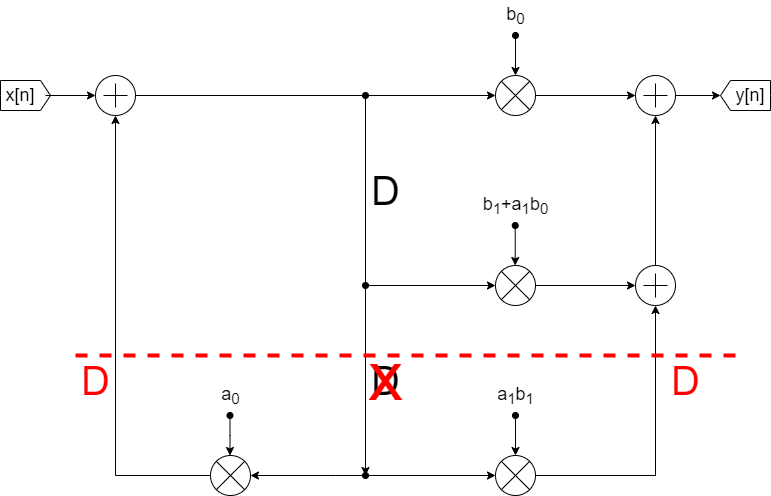
\includegraphics[width=0.55\textwidth]{IIR_2_1.png}
	\caption{Advanced architecture with $1^{st}$ transformation}
	\label{fig:IIR_advanced_2}
\end{figure}

In \autoref{fig:IIR_advanced_3} a feed-forward cut-set has been identified where it is possible to insert a pipeline stage on all three branches. In this way the combinatorial path including the $b_0$ multiplier is no longer part of the critical path. The longest combinatorial path includes the multiplier for the term $b_1 + a_1b_0$, the intermediate adder and the final adder. A further transformation allows to move the register from one side of the multiplier to the other without altering the behavior of the circuit, as in \autoref{fig:IIR_advanced_4}.

\begin{figure}[ht]
	\begin{minipage}[b]{0.5\linewidth}
		\centering
		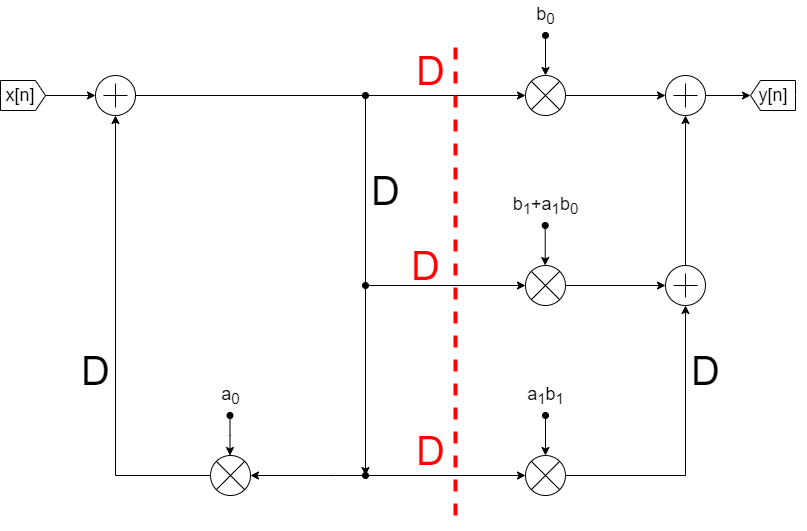
\includegraphics[width=\textwidth]{IIR_2_2.png}
		\caption{Advanced architecture with $2^{nd}$ transformation}
		\label{fig:IIR_advanced_3}
	\end{minipage}
	\hspace{0.5cm}
	\begin{minipage}[b]{0.5\linewidth}
		\centering
		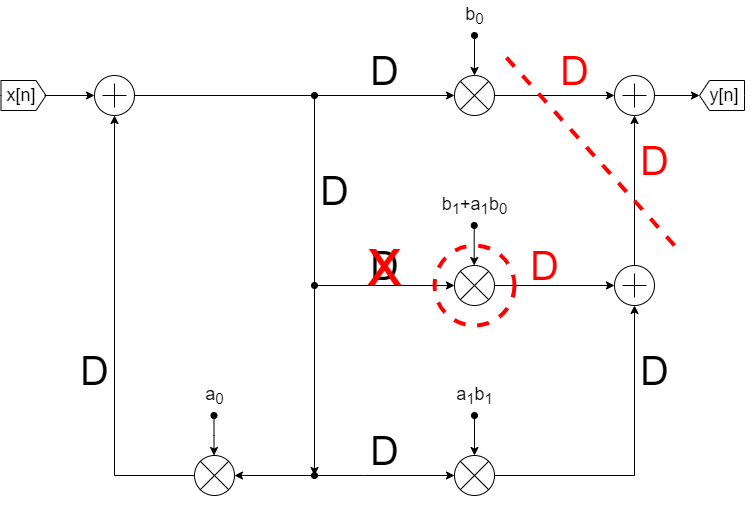
\includegraphics[width=\textwidth]{IIR_2_3.png}
		\caption{Advanced architecture with $3^{rd}$ transformation}
		\label{fig:IIR_advanced_4}
	\end{minipage}
\end{figure}

The latter transformation in \autoref{fig:IIR_advanced_4} takes into account the feed-forward cut-set on the two input branches at the last adder and through the insertion of a pipeline stage bring the critical path to be equal to the delay of a single multiplier.

In \autoref{fig:IIR_final} the optimized architecture of the IIR filter can be observed, in which a pipeline stage has been inserted between each combinatorial block. These transformations allow the circuit to reach the maximum throughput at the expense of latency, which compared to the initial circuit has increased from $2\,T_{ck}$ to $4\,T_{ck}$. 

\begin{figure}[htb]
	\center
	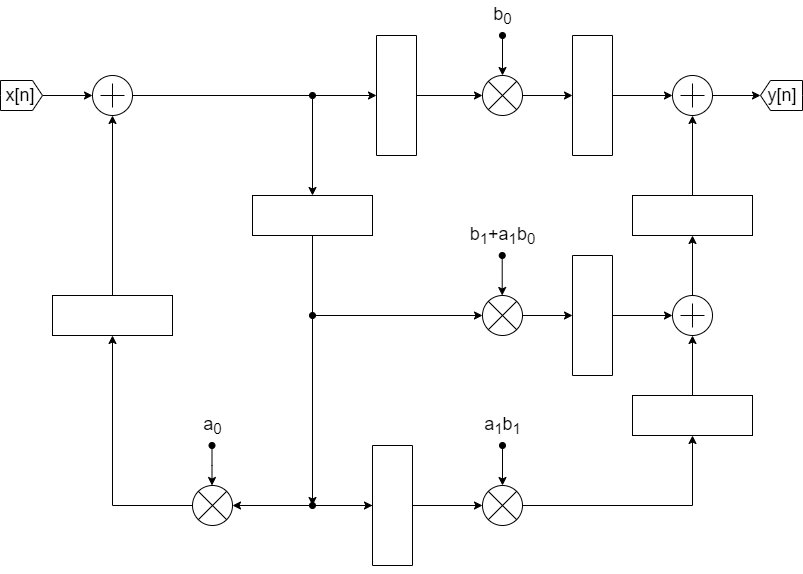
\includegraphics[width=0.65\textwidth]{IIR_final.png}
	\caption{Optimized architecture of J-look-ahead IIR filter}
	\label{fig:IIR_final}
	\end{figure}

\pagebreak

\subsection{Simulation}
For the simulation of the circuit has been used the same testbench since the external entity of the circuit has not been modified with respect to the previous implementation.
In \autoref{fig:wave_start_j} the timing with the signals of the DUT is shown.In this case when the $VIN$ signal becomes valid 4 clock periods are required until the first result is available at the output; the explanation for this longer latency is due to the pipeline stages introduced in the circuit.

\begin{figure}[h]
	\center
	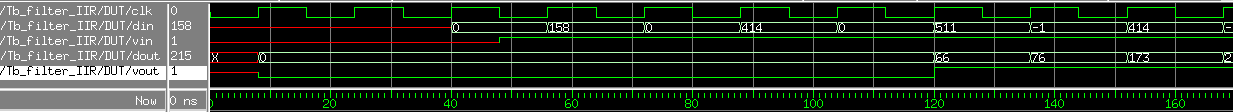
\includegraphics[width=1\textwidth]{images/wave_start_j_look_ahead.png}
	\caption{Start of the simulation}
	\label{fig:wave_start_j}
\end{figure}

Finally in \autoref{fig:wave_vin_j} it is observed the correct operation of the circuit when $VIN$ becomes low and then high. The internal registers do not sample when $VIN$ is not asserted, so the output data does not change, keeping the output valid. When $VIN$ returns to $1$, only one clock period is required before the output changes value because the registers are already full. 

\begin{figure}[h]
	\center
	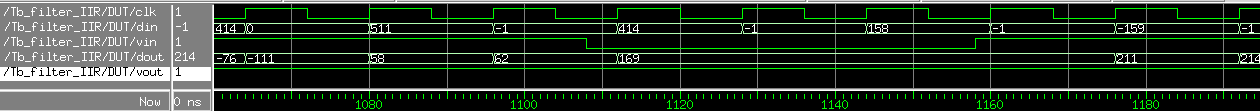
\includegraphics[width=1\textwidth]{images/wave_vin_0_1_j_look_ahead.png}
	\caption{Simulation of $VIN$ signal trnsition}
	\label{fig:wave_vin_j}
\end{figure}

Once the correct timing of the circuit has been verified, the output data has been compared with the corresponding C implementation of the realized model. With the same set of data used for the testbench of the previous architecture, the same output results were obtained. You can refer to the data shown in \autoref{tab:tab_results} to have an outline of the results.


\subsection{Logic Synthesis}
Having verified the correct functioning of the filter with Modelsim, Synopsys has been used for synthesis. The objective is to calculate the maximum frequency of operation of the circuit and then setting $T_{CLK} = 4 T_{min}$, compute the area and the dissipated power, using the data on switching activity produced by Modelsim.
The results related to the clock period, the associated slack and the area are shown in \autoref{tab:timing_rep_j}.

\begin{table}[h]
\begin{center}
\begin{tabular}{|l|l|l|}
\hline
$T_{CLK}$ (ns) & slack (ns) & area $(\SI{}{\micro\meter})^2$ \\
\hline
10 & 7.39 &  3200\\
0 & -1.75 &  3834\\
2.15 & 0 & 3542 \\
8.6 & 5.99 & 3200 \\
\hline
\end{tabular}
\end{center}
\caption{Results of timing report}
\label{tab:timing_rep_j}
\end{table}

Subsequently the netlist generated was used to determine the switiching activity using Modelsim and obtain in this way an accurate estimation of the power consumption of the circuit. The results are shown in \autoref{fig:pow_rep_x4_j}.

\begin{figure}[h]
	\center
	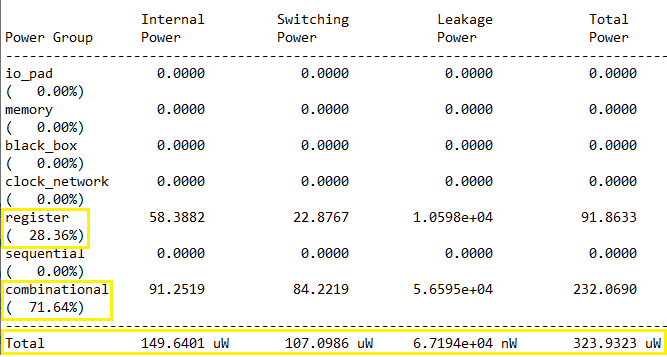
\includegraphics[width=0.8\textwidth]{images/report_power_x4_j_mod.png}
	\caption{Power Report}
	\label{fig:pow_rep_x4_j}
\end{figure}

Also in this case it is noted that the power consumption is mainly produced by the combinatorial part consisting of 3 adders and 4 multipliers.

\subsection{Place \& Route}
The Place \& Route with the innovus software has been carried out following the previous procedure. The generated circuit is the one shown in \autoref{fig:layout_j}, it has an area equal to $\SI{3186}{\micro\meter}^2$ according to the one obtained from the Synopsys report, with a total of 1588 cells and 3993 gates. The values obtained are plausible if compared to those of the previous architecture because in this case there are more physical elements (registers, summers and multipliers) and consequently the need for more area to allocate all the necessary gates is expected.

\begin{figure}[h]
	\center
	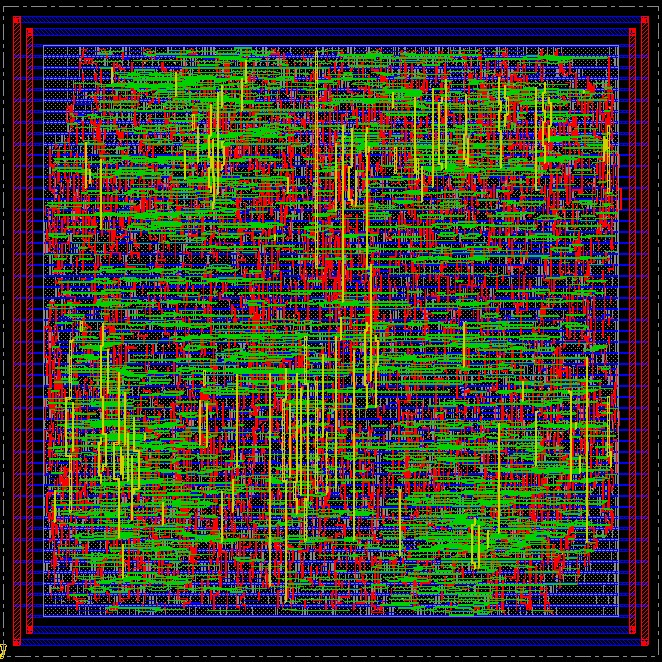
\includegraphics[width=0.6\textwidth]{images/IIR_filter_period_min_x4_place_j.jpg}
	\caption{Resulting layout}
	\label{fig:layout_j}
\end{figure}

Subsequently it was launched the timing analysis, the verification of connectivity and geometry, which showed the absence of any violation. Starting from the switching activity data obtained from Modelsim, an estimation of the power has been performed. The results are shown in \autoref{fig:cadence_pow_rep_x4_j}, also in this case the results obtained are in line with those obtained from the Synopsys power report.

\begin{figure}[h]
	\center
	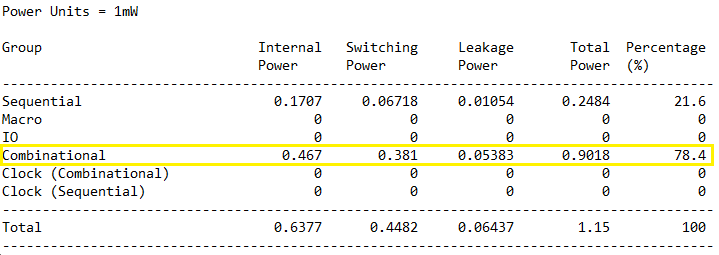
\includegraphics[width=0.8\textwidth]{images/rep_power_x4_cadence_j_mod.png}
	\caption{Post place \& route power report}
	\label{fig:cadence_pow_rep_x4_j}
\end{figure}
>>>>>>> 293cc19a93f5661c8a6b7317d24476e5716826e5
